% =============================================================================
% Kapitel 4: Testplanung und -durchführung 
% =============================================================================

\chapter{Testplanung und -durchführung}

\section{Funkabdeckungstest}

\subsection{Auswahl der Gateways}

Um eine systematische Untersuchung der Funkabdeckung im urbanen Raum durchführen zu können, wurden zunächst geeignete Gateways 
identifiziert, um die herum die Testrouten konstruiert werden sollten. Als Grundlage diente die öffentlich zugängliche 
Abdeckungskarte von TTN Mapper, die sowohl die Standorte registrierter Gateways als auch eine Heatmap historisch 
beobachteter Signalstärken anzeigt. 

\begin{figure}[H]
    \centering
    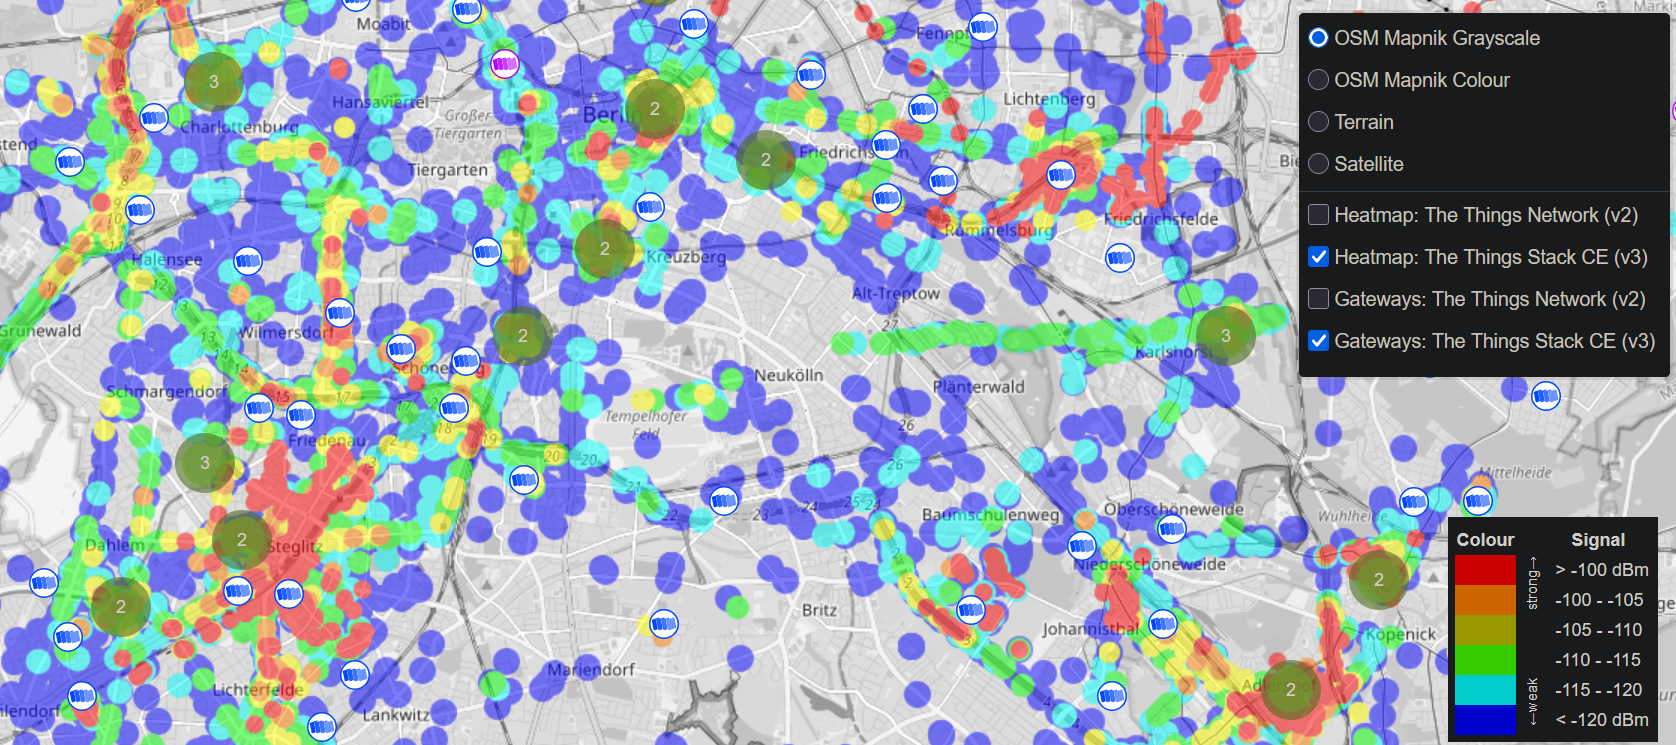
\includegraphics[width=\textwidth]{kapitel4/pictures/ttn_mapper_berlin.png} 
    \caption{Übersicht TTN-Gateways in Berlin}
    \label{fig:ttn_mapper}
\end{figure}

Abbildung \ref{fig:ttn_mapper} verdeutlicht verschiedene Clusters, wo die empfangene Signalstärke im 
roten Bereich liegt. Dazu zählen insbesondere die Ballungsräume
um den Bahnhof Lichtenberg, den Campus der TU-Berlin in Charlottenburg, die Zentrallandesbibliothek (ZLB) Mitte, 
sowie den Bahnhof Rathaus Steglitz. Gateways an den beiden letztgenannten Orten eignen sich ideal für eine Testkampagne: 3 Gateways in 
Steglitz gehören zu den höchstplatzierten im Raum Berlin und Brandenburg (s. Tabelle \ref{tab:gateway_info}), weshalb mit ihnen das Erreichen
maximaler Funkreichweiten evaluiert werden soll. Das Gateway in Mitte stellt hierzu den Gegenpol dar:
es verfügt über eine geringe Montagehöhe wurde aufgrund seiner unmittelbaren Nähe zum primären Forschungsstandort ausgewählt.

\begin{table}[htbp]
    \centering
    \caption{Für Feldtests ausgewählte TTN-Gateways.}
    \label{tab:gateway_info}
    \begin{tabular}{lccc}
        \toprule
        \textbf{Gateway-ID} & \textbf{Breitengrad} & \textbf{Längengrad} & \textbf{Höhe} \\
        \midrule
        zlb-ttn-in-02 & \SI{52.516169}{\degree} & \SI{13.404518}{\degree} & \SI{12}{\meter} \\
        pattilux-gateway & \SI{52.450619}{\degree} & \SI{13.321081}{\degree} & \SI{80}{\meter} \\
        ttn-outdoor-02 & \SI{52.457873}{\degree} & \SI{13.310390}{\degree} & \SI{90}{\meter} \\
        eui-a84041ffff252dac & \SI{52.468846}{\degree} & \SI{13.305556}{\degree} & \SI{60}{\meter} \\
        \bottomrule
    \end{tabular}
\end{table}